\chapter{Method}

This chapter will introduce and develop the \rrtfunnel\ algorithm, through two
means: Developing robust motion primitives through the \ac{SOS} programming
framework, based on the work in~\cite{majumdarFunnelLibrariesRealtime2017}, and
second deploy these funnels as motion primitives in a discrete \ac{RRT} planner,
based on~\cite{lavalleLav98cPdf}. This is beneficial, as using \textit{robust}
motion primitives has several advantages. Firstly, they are robust to
uncertainty, and thus, as long as the uncertainties in the system are akin to
our assumptions, the vehicle will not leave the funnel. Secondly, with the
assumption that the primitives are robust, there is no need for more
conservative maneuvers and heuristics, such as maximizing the distance to an
obstacle. This means that a robust motion primitive algorithm can perform more
aggressive maneuvers than one that is inherently cautious about its
environment~\cite{majumdarFunnelLibrariesRealtime2017}.

\section{The funnel part}

In order to create a basic set of funnels as the robust motion primitives for
the \rrtfunnel{} motion planning algorithm, a few obstacles have to be overcome
first. The first one is settling on a model for the funnel calculations. This
thesis is using the simple car model from \cite[LaValle.p~613]{Lav06} which is
modified slightly into
\begin{equation}
  \label{eq:model-dynamics}
  \mathbf{x} =
  \begin{bmatrix}
    x \\ y \\ \theta \\ \dot{\theta} \\
  \end{bmatrix}, \, \dot{\mathbf{x}} =
  \begin{bmatrix}
    -v(t)\sin(\theta) \\
    v(t)\cos(\theta) \\
    \dot{\theta} \\
    u \\
  \end{bmatrix},
\end{equation}
which is a second-order unicycle model with constant speed. A picture of the
model can be found in figure~(\ref{fig:second-order-unicycle}).
\begin{figure}
  \centering \resizebox{10em}{!}{
    \import{figures/method/}{unicycle-model.pdf_tex} }
  \caption{The unicycle model of a vehicle.}
  \label{fig:second-order-unicycle}
\end{figure}
Although this is the only model used in this thesis, the framework and the code
is easily adapted into accommodating a different and more complicated model for
planning.


\subsubsection{Generating the trajectories}

The trajectories are generated through the \textit{Direct collocation method}.
This is choses because it fits well with the sampling that is done along the
nominal trajectory for in this case, optimal trajectory planning, but also fits
well with the sampling that is done when generating the invariant regions around
the sampled paths along the trajectory for the funnel generation. The chosen
method is nonlinear, and any other number of methods could have been used in
order to generate the initial trajectories, however the direct collocation
method filled the needs for the initial trajectory library well.

Since it is an optimal trajectory planner, a cost function has to be chosen for
the solver to minimize. The cost function of the type
\begin{equation}
  J = \int_{0}^{T} \left[ 1 + {u_{0}}^{T}Ru_{0} \right] dt
\end{equation}
from~\cite{majumdarFunnelLibrariesRealtime2017} was chosen as it gives the
vehicle a dependence upon the input, and will generate input graphs, which is
beneficial for not having the vehicle act too aggressively, while it also gives
a depence upon the time spent.

An initial trajectory set is pictured in~\ref{fig:initial-trajectories}, and
consists of a left-turn, a straight-forward, and a right-turn motion.

\begin{figure}
  \centering
  \begin{minipage}[b]{0.2\textwidth}
    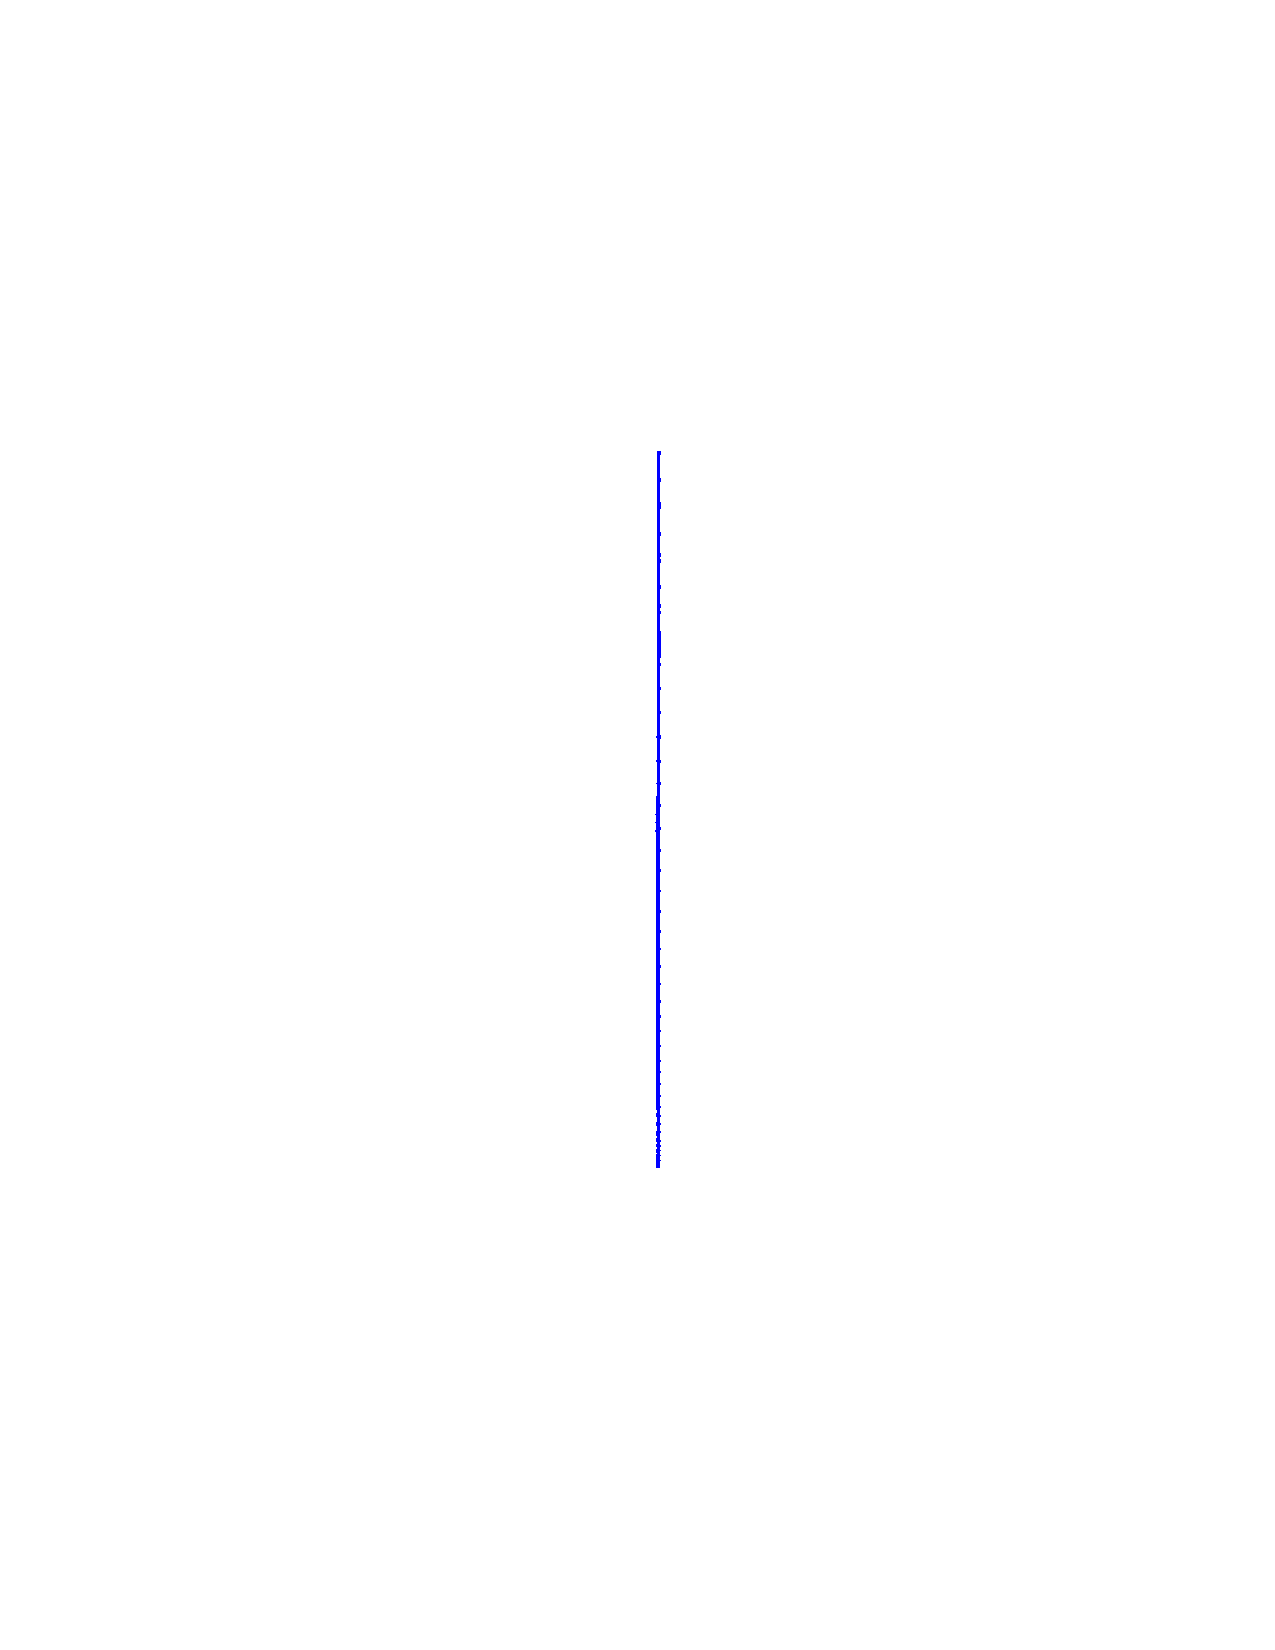
\includegraphics[width=\textwidth]{figures/method/straight-trajector}
  \end{minipage}
  \hfill
  \begin{minipage}[b]{0.2\textwidth}
    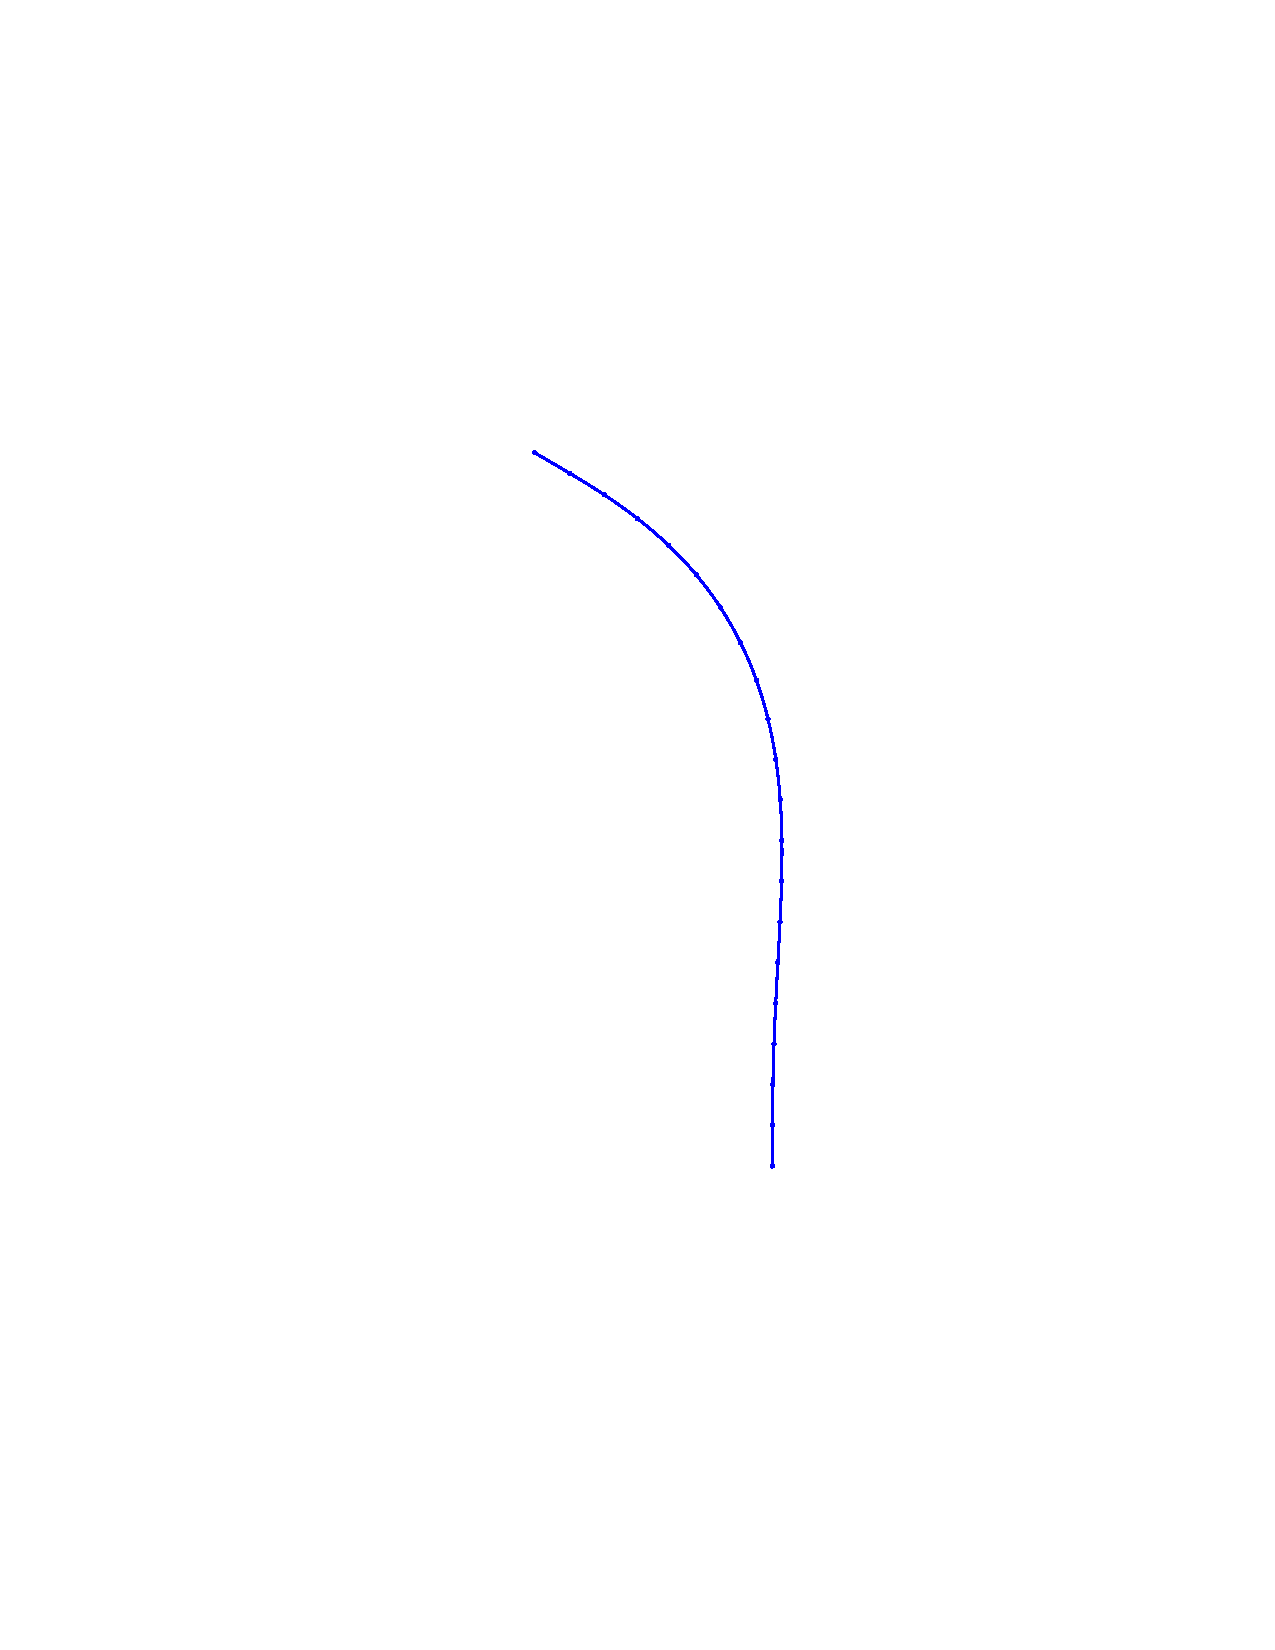
\includegraphics[width=\textwidth]{figures/method/left-trajector}
  \end{minipage}
  \hfill
  \begin{minipage}[b]{0.2\textwidth}
    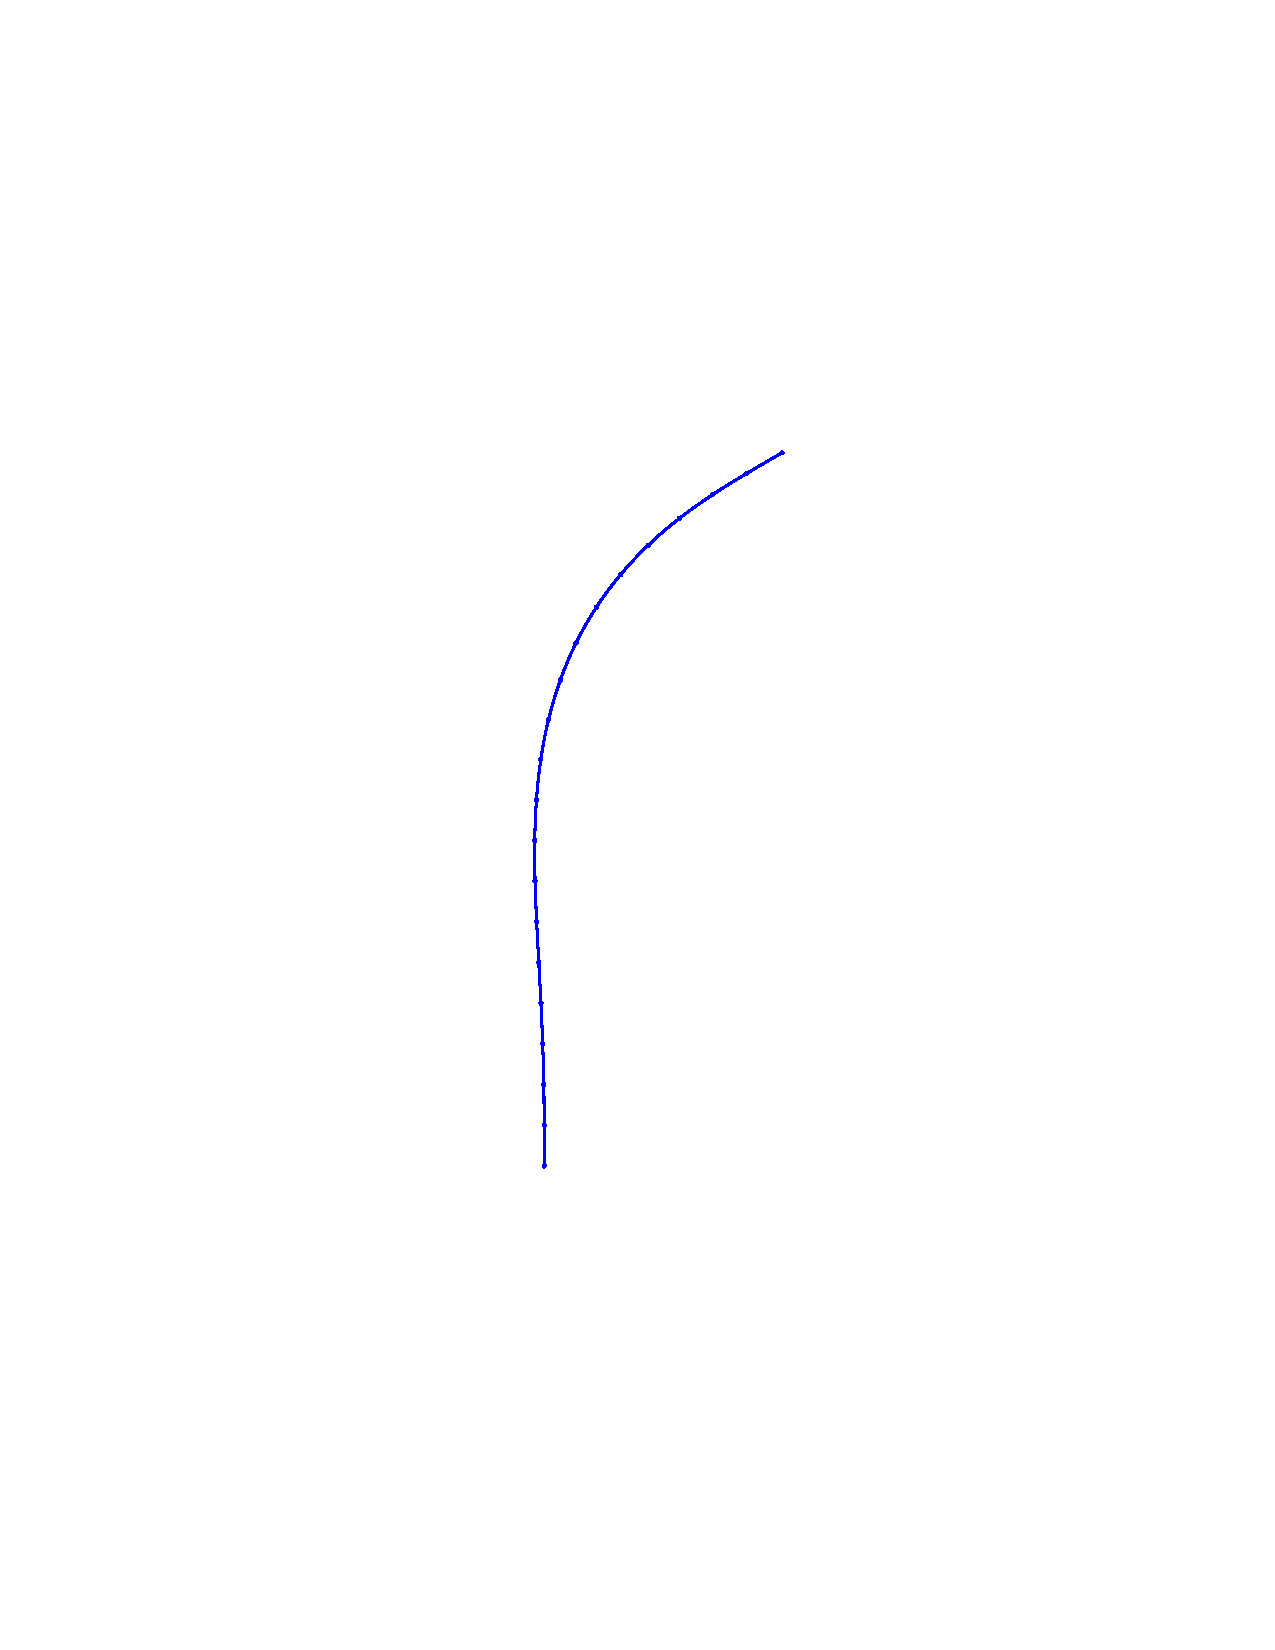
\includegraphics[width=\textwidth]{figures/method/right-trajector}
  \end{minipage}
  \caption{Three motion primitives for the \rrtfunnel{} algorithm, one
    straight, one left, and one right turn.}
  \label{fig:initial-trajectories}
\end{figure}

TODO - maybe add the initial point generation algorithm here?

\subsubsection{Initializing the funnel calculations with a TVLQR candidate as
  the initial Lyapunov function}

The funnel calculation algorithm has to be initialized with a Lyapunov candidate
in the same way as~\cite[Majumdar]{majumdarFunnelLibrariesRealtime2017}, the
funnel generation algorithm will be initialized with a \ac{TV-LQR} controller,
employing a cost function of the form
\begin{equation}
  J = x^{T}(t_1)F(t_1)x(t_1) + \int_{t_{0}}^{t_{1}} \left( x^{T}Qx + u^{T}Ru + 2x^TNu \right) \mathrm{dt},
\end{equation}
which when employed on the linearization of the system dynamics
\begin{equation}
  \dot{\bar{x}} \approx A(t)\bar{x}(t) + B(t)\bar{u}(t) +D(t)w(t),
\end{equation}
gives an initial candidate Lyapunov function
\begin{equation}
  V(t,x) = {\bar{x}}^{T}S_{i}\bar{x}.
\end{equation}

Although the focus of this thesis is not on fine-tuning the controller, some
amount of effort has to go into getting the cost parameters acceptable. In
general the strategy is penalizing the vehicle's distance from the nominal path
in \((x,y,\theta)\), and not caring for the energy expended by the control
input. Thus path divergence is penalized hard, and input divergence is not. More
specifically the cost matrices employed are
\begin{align*}
  R &= 0.01 \\
  Q &= \begin{bmatrix}
    40 & 0 & 0 & 0 \\
    0 & 40 & 0 & 0 \\
    0 & 0 & 40 & 0 \\
    0 & 0 & 0 & 4 \\
  \end{bmatrix}
  \\
  Q_{f} &=
          2\times
  \begin{bmatrix}
    1 & 0 & 0 & 0 \\
    0 & 1.5 & 0 & 0 \\
    0 & 0 & 1 & 0 \\
    0 & 0 & 0 & 1 \\
  \end{bmatrix}
\\
\end{align*}
where the control input is only penalized \(\frac{1}{10}\)th of the other
variables.

\subsubsection{Generating the funnels around the trajectories}

With the nominal trajectories, and the initial Lyapunov functions now ready, the
funnels around the nominal trajectories can be calculated using the
algorithm~\ref{alg:funnelalgorithm}. % The implementation is an expansion upon
% code from the~\cite[Drake toolbox]{drake}, whereas the \ac{SOS} implementation
% is kicked out to a \ac{SOS} solver built upon~\[sostools\]\cite{sostools}.

However, two obstacles remains, as the dynamics for the
model~\ref{eq:model-dynamics} are still not polynomial. Thus in order to obtain
the needed polynomial dynamics, the system is expanded around the nominal
trajectory with a Taylor expansion of degree three. Secondly the function
limiting the size of the funnel \(\rho(t_{k})\) has to be initialized by a
feasible \(\rho(t)\) as well. This is done through the equation
\begin{equation}
  \rho(t_{k}) = \mathrm{exp}\left( \rho_{\tau}\frac{\left( t_{f} - t \right)}{\left( t_{f} - t_{0}  \right)}\right)
\end{equation}
from~\cite[eq.~6.sec~3]{tobenkinInvariantFunnelsTrajectories2010}. Where
\(\rho_{\tau}\) is a positive constant determining the upper bound on the
funnel. If the given choice of \(\rho_{\tau}\) does not verify a funnel, either
increase the value of \(\rho_{\tau}\), and optionally the number of sampled
points from the trajectory to be
verified~\cite{tobenkinInvariantFunnelsTrajectories2010}.

Thirdly, the initial condition set has to be decided beforehand. In general the
initial condition set can be any semi-algebraic set in the state-space. However,
a simple way of obtaining a initial condition set for the trajectories at hand
is by taking advantage of the Lyapunov function canditate from the
\ac{LQR}-controller. Thus by setting
\begin{equation}
  \mathcal{X}_{0} = \frac{S_{k}}{\rho_{\tau}}
\end{equation}
an intial condition is obtained. For the controller

For the cost function in the funnel generation
algorithm~\ref{alg:funnelalgorithm}, which in general is a maximization of the
determinant of the upper bound ellipse for the funnel set, a weight is added to
each element in order to further fine-tune the size of the funnel. As an
example: For the vehicle model in this thesis the size of the funnel projected
down into the xy-plane will be the most important metric. Whether or not the
vehicle's orientation parameter \(\theta\) is close to the nominal heading is of
less concern, and is therefore down-prioritized, along with the cost on the
control input \(u\). Having a large \(\theta\) and \(\dot{\theta}\) semi-axis in
the hyperellipsoid can also be beneficial, as it increases the inlet of the
ellipsoid at hand. All this taken together then gives the cost function
\begin{equation}
  P_{k} = W_{k}P_{k}W_{k}^{T}
\end{equation}
where
\begin{equation}
  W_{k} =
  \begin{bmatrix}
    10 & 0 & 0 & 0 \\
    0 & 10 & 0 & 0 \\
    0 & 0 & 1 & 0 \\
    0 & 0 & 0 & .1 \\
  \end{bmatrix}
\end{equation}

\begin{figure}
  \centering
  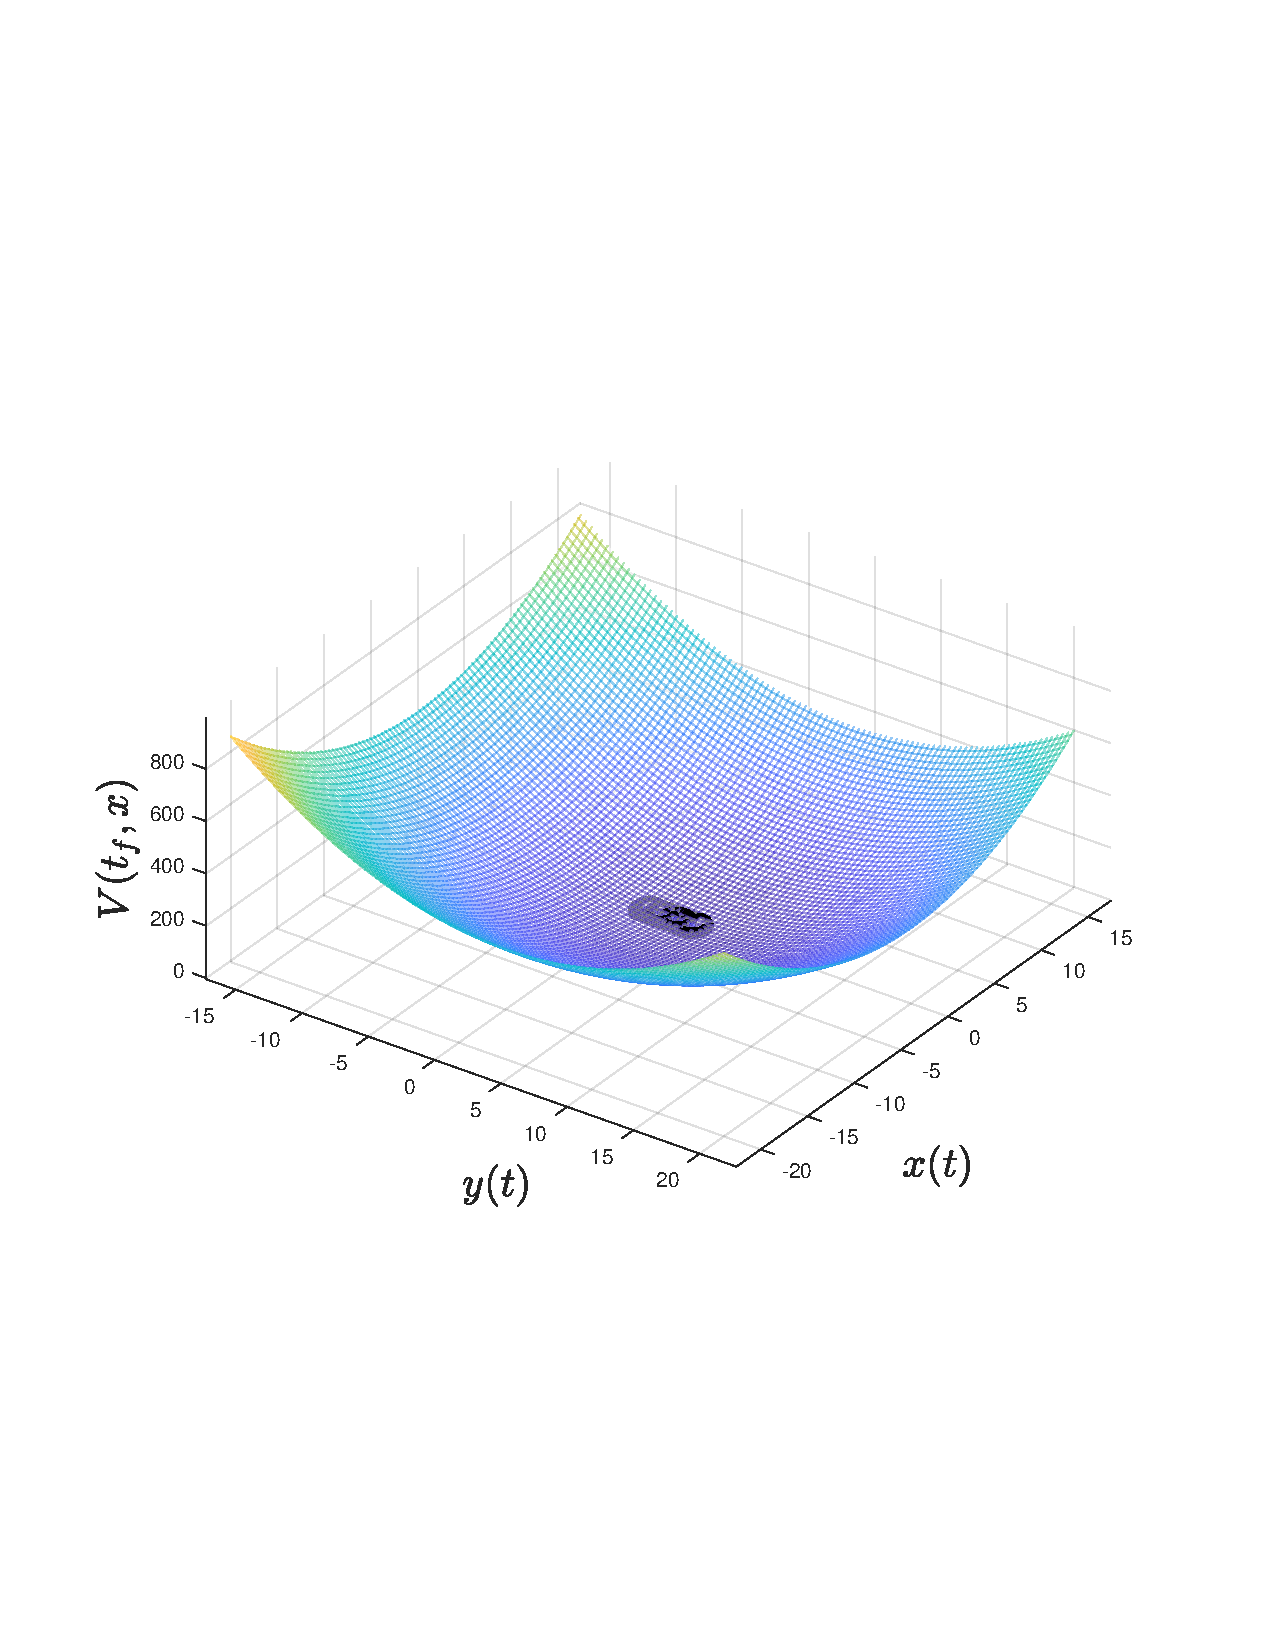
\includegraphics[scale=.3]{figures/rrtfunnel/straight-funnel-lyapunov-3d}
  \caption{A visualization of the Lyapunov function values around a straight
    motion primitive.}
  \label{fig:visualized-lyapunov}
\end{figure}

\subsection{Adding uncertainty to the funnel calculation}
\label{sec:adding-uncertainty}

Following are the changes to the formulations so that a funnel takes into
account a bounded uncertainty term of the form \(\mathcal{W} = \set{ w(t) \in
  R^d \mid g_{w,j}(w) \geq 0 \forall j = 1,\ldots,N_w}\). Adding an extra term
to the closed-loop dynamics equation
\[
  \dot{\bar{x}} = f_{cl}(t, \bar{x}(t), w(t))
\]
the requirement~(\ref{eq:reachableset}) is slightly modified so that
\begin{equation}
  \label{eq:uncertain-reachableset}
  \bar{x}(0) \in \mathcal{X} \implies \bar{x}(t) \in F(t),\, \forall t \in
  [0,T], \, \forall w \colon [0,T] \rightarrow \mathcal{W}
\end{equation} 
\(F(t)\) is the new reachable set for the uncertain system. Thus the sufficient
condition~(\ref{eq:funnelsufficient}) turns into
\begin{equation}
  \label{eq:funneluncertain-sufficient}
  V(t,\bar{x}) = \rho(t) \implies \dot{V}(t,\bar{x},w) < \dot{\rho}(t), \, \forall t \in [0,T], \, \forall w(t) \in \mathcal{W}.
\end{equation}
The Lyapunov function is calculated as
\begin{equation}
  \dot{V}(t,\bar{x}, w) = \frac{\partial V(t,\bar{x})}{\partial x} f_{cl}(t,\bar{x},w) + \frac{\partial V(t,\bar{x})}{\partial t},
\end{equation}
and the optimization condition~(\ref{eq:optimizationconditionsos}) turns into
\begin{align}
  \label{eq:optimizationconditionuncertain}
  \dot{\rho}(t) - \dot{V}(t,\bar{x},w) - L(t,\bar{x},w) \left[ V(t,\bar{x}) - \rho(t) \right] - L_{t}(t,\bar{x},w)\left[ t\left( T - t \right) \right]  & \nonumber \\
  - \sum_{j=1}^{N_{w}} L_{w,j}(t,\bar{x},w)g_{w,j}(w) \quad \text{is SOS} &  \\
  \L_{w,j}(t,\bar{x},w) \qquad \text{is SOS}, \; \forall j = 1,\ldots,N_w \nonumber
\end{align}

All this is to be cited to~\cite{majumdarFunnelLibrariesRealtime2017}.

\subsubsection{Shifting funnels and invariance}

In order to freely shift funnels around in the configuration space, the cyclic
coordinates of the system has to be determined. ex:
\begin{align}
  \mathcal{L} &= T - V = \frac{1}{2} mv^2 + \frac{1}{2}I\dot{\theta}^2 \\ 
              &= \frac{1}{2} 
                m\begin{bmatrix}
                  -v\sin \theta \\ 
                  v \cos \theta \\
                \end{bmatrix}^{T}
  \begin{bmatrix}
    -v\sin \theta \\
    v \cos \theta \\
  \end{bmatrix}
  + I\dot{\theta}^2 \\
              &= m \left(
                v^2 \sin^2 \theta + v^2 \cos^2
                \right)  + I {\dot{\theta}}^2 \\
              &= mv^2 + I {\dot{\theta}}^2 \\
\end{align}
which shows that the LaGrangian is invariant to shifts in the \((x,y,\theta)\)
variables, since \(\frac{\partial\mathcal{L}}{\partial q_i} = 0 \, q_i =
x,y,\theta\). Hence now, any funnel in the base set can be shifted around, and
thus create an infinite set of funnels in the state space. Through the
partitioning of coordinates into cyclic- and non-cyclic coordinates, of the form
\(x = [x_c x_{nc}]\), the state dynamics \(\dot{x} = f(x(t), u(t))\) only
depends on the non-cyclic coordinates of the system. Thus, a trajector of the
form \(t \rightarrow (x(t),u(t))\) which solves \(\dot{x} = f(x(t),u(t))\) can
then be transformed through a shift \(\Psi_c\) along the cyclic coordinates of
the system to yield a valid solution of the form
\[
  t \rightarrow (\Psi_{x}(x(t)), u(t))
\]
which is a trajector shifted to a different place in the state space, but is
still valid. The transform \(\Psi\) is given by
\[
  \Psi([x_c, x_{nc}]) =  
  \begin{cases}
    x_c \rightarrow \hat{x}_{c} \\
    x_{nc} \rightarrow x_{nc} \\
  \end{cases}.
\]

\subsection{Checking which funnels can be composed and not}
\label{sec:composable-funnels}

Now that funnels can be shifted freely around the state space to create new
motion primitives it is time to chain funnels together to create chains, and
eventually trees of funnels that span out into the planning environment to
create robust maneuvers that the vehicle can follow. An abstract pictorial
representaion of two funnels composed together can be seen
in~(\ref{fig:two-funnels-composed}). The mathematical definition of funnel
composition~(\ref{def:funnel-composition}), is used to verify that two funnels
are composable, and implemented as a \ac{SOS}-program which can be found
in~(\ref{AppendixB}). However, take note that the definition has to be modified
slightly in order to take into account the translation along the cyclic
coordinates. Hence the definition used
is~\cite[definition~3,sec~5]{majumdarFunnelLibrariesRealtime2017} which states
\begin{definition}
  An ordered pair \(F_1,F_2\) of funnels \(F_1 \colon [0,T_1] \rightarrow
  \mathcal{P}(\R^n)\) and \(F_2 \colon [0,T_2] \rightarrow \mathcal{P}(\R^n)\)
  is \textit{sequentially composable modulo invariances} if there exists a shift
  along cyclic coordinates such that \(F_{1}(T_1) \subset
  \Psi_{c}\left(F_2(0)\right)\)
\end{definition}
In laymans terms this means that if a funnel \(F_2\) can be shifted along cyclic
coordinates to stack up against the outlet of funnel \(F_2\) so that they are
composable in the sense of definition~(\ref{def:funnel-composition}). Hence,
basically any funnel in the state space can be seen as a set consisting of the
funnel from the basic set, along with a transformation along the cyclic
coordinates of the system \(F_n \in \R^n \mid \Psi_{c,i}(F_i), F_i \in
\mathcal{F}\), where \(\mathcal{F}\) is the basic set of funnels.

\begin{figure}
  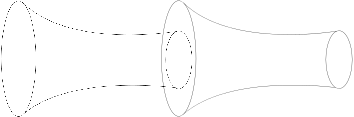
\includegraphics[scale=.2]{figures/method/funnel-composition} \centering
  \caption{Two funnels composed.}
  \label{fig:two-funnels-composed}
\end{figure}

Using the generalized S-procedure the condition
\begin{equation}
  V_1(T_1,\bar{x}) \leq \rho_1(T_1) \implies V_2(0, \bar{x}) \leq \rho_2(0)
\end{equation}
the composability of the funnels can be checked through the \ac{SOS} program
\begin{align*}
    & \text{Find } && L(\bar{x}) \\
    & \text{s.t. } && \rho_2(0) - V_2(0,\bar{x}) - L(\bar{x})\left( \rho_1(T_1) - V_1(T_1,\bar{x}) \right) \text{ is SOS} \\
    &&& L(\bar{x}) \text{ is SOS} \\
\end{align*}

\subsection{Only minimizing the volume of the funnel projected down into the
  xy-plane}

There is no need in minimizing the value of \(\dot{\theta}\), so in order to
minimize what we care about, i.e. the actual size of the funnel where the
physical vehicle can move, we modify our costfunction according to
\cite{majumdarFunnelLibrariesRealtime2017}. Thus, given a projection map \(\pi :
\R^n \rightarrow \R^{n_p}\). Given the ellipsoid \(\epsilon = \set{\bar{x} \in
  \R^n | \bar{x}^TS_{k}\bar{x} \leq 1}\) with
\[
  S_k^{(p)} = \p{PS_k^{-1}P^T}^{-1}
\]
Given that minimizing the volume of the ellipsoid \(\epsilon\) using an SDP
relies on maximizing the determinant of \(S_k\). Since \(det(S_k)\) is a
nonlinear function of \(S_k\), the function has to be linearized in order for it
to be handled by our solution framework (SOS-programming).
\cite{majumdarFunnelLibrariesRealtime2017} solves this by linearizing
\(det(S_k)\) at the solution of \(S_k\) from the previous iteration, and
maximizes this linearization instead. In the end this translates to
\[
  lin\p{det\p{S_k}} =
  Tr\p{P^T\p{PS_{k,0}^{-1}P^T}^{-1}PS_{k,0}^{-1}S_kS_{k,0}^{-1}}
\]
where \(S_{k,0}\) is the nominal value.

\subsection{Searching for a controller which minimizes the size of the funnel}

With the non-optimal feedback controller given to the funnel calculation
framework, the size of the funnels will in general be larger than they could
have been if given a better controller. This is not beneficial given that the
funnels is going to be used as motion primitives for an algorithm planning in a
dense forest. Hence, referring to~\cite[Majumdar.sec~4.3.2 (Feedback control
synthesis)]{majumdarFunnelLibrariesRealtime2017}, the initial controller input
to the algorithm can be optimized with the goal of minimizing the size of the
funnel, given a few conditions on the system.

Firstly the system needs to be control affine:
\begin{equation}
  \dot{x} = f(x(t)) + g(x(t))u(t)
\end{equation}
so that the control policy can be parametrized as a polynomial
\(\bar{u}_f(t,\bar{x})\), and the system dynamics written as:
\begin{equation}
  \dot{\bar{x}} = f(x_0(t) + \bar{x}(t)) + g(x(t))\left[ u_0(t) + \bar{u}_f(t,\bar{x}) \right] - \bar{x}_0
\end{equation}
Then the feedback controller can be optimized by adding the coefficients of the
polynomial \(u_f(t,\bar{x})\) to the set of decision variables in the original
optimization problem. The only issue is that now \(\dot{V}\) is bilinear in the
decision variables
\begin{equation}
  {
    % \newcommand{\x}{\bar{x}}
    \newcommand{\Vdot}{\dot{V}}
  \Vdot(t,\x) = \frac{\partial V(t,\x)}{\partial \x} \dot{\x} + \frac{\partial V(t,\x)}{\partial t}
  }
\end{equation}
In order to minimize the cost function a search is done in
\((\bar{u}_f,\rho,L_t,L_{0,i},S_k)\) while keeping \((V,L,L_{\epsilon,k})\)
fixed. This method combined with the uncertainty added
in~(\ref{sec:adding-uncertainty}), is what is the basis of the funnel
computations in this thesis as summarized in algorithm~(\ref{alg:funnelalgorithm-extended}).

\begin{algorithm}[H]
  \caption{Feedback Funnel computation}
  \label{alg:funnelalgorithm-extended}
  \DontPrintSemicolon \SetAlgoNoLine

  \KwIn{\(V\) and \(\rho\)} \KwOut{Funnel}

  \(cost_{prev} = \infty\)\; converged = false \; \While{\(\neq converged\)}{
    Optimization problem 1: \;
    \begin{align*}
      \underset{\substack{\bar{u}_f,L,L_{t},L_{0,i},S_{k},L_{}}}{\inf}&  \sum_{k=1}^{N} \vol(\mathcal{E}(t_{k}))& \\    
      \text{subject to } & V \text{ and } \rho \text{ constant.}& \\
    \end{align*}\;
    Optimization problem 2: \;
    \begin{align*}
      \underset{\substack{\bar{u}}_f,\rho,L_{t},L_{0,i},S_{k}}{\inf}&  \sum_{k=1}^{N} \vol(\mathcal{E}(t_{k}))& \\    
      \text{subject to } & (V,L,L_{\mathcal{E},k}) \text{ constant.}& \\
    \end{align*}\;
    Optimization problem 3: \;
    \begin{align*}
      \underset{\substack{V,\rho, L_{t},L_{0,i},S_{k}}}{\inf}&  \sum_{k=1}^{N} \vol(\mathcal{E}(t_{k}))& \\    
      \text{subject to } & (L,L_{\mathcal{E},k},\bar{u}_f) \text{ constant.}& \\
    \end{align*}\;
    cost = \(\sum_{k=1}^{N} \vol(\mathcal{E}(t_{k}))\) \;
    \If{\(\frac{cost_{prev} - cost}{cost_{prev}} < \epsilon\)} {
      converged = true
    }\;
    \(cost_{prev} = cost\)\;
  }\;
\end{algorithm}

\section{RRT}

With the basic framework for dealing with funnels as motion primitives
constructed, it is time to build the \ac{RRT} part of the \rrtfunnel{}
algorithm. The reason for choosing to base the global path planning framework on
the \ac{RRT} motion planning algorithm are as follows. One, it has the ability
ot quickly expand deep into the search-space, and then later progress towards a
finer sampling, which is valuable as it avoids local minima. The \ac{RRT} is
also relatively simple to implement, and has only three main components that
needs to be in place in order for successful path planning to happen in an
arbitrary state space.

\subsection{Uniform sampling in SO(2)}

One, as mentioned in~(\ref{sec:rrt-sampling}), the \ac{RRT} algorithm needs
uniform sampling of the state space in order for it to function optimally. As
over- or under-sampling certain parts of the state space can lead to poor
performance.

From~\cite{kuffnerEffectiveSamplingDistance2004} the samples can be generated
uniformly on the Euclidean plane through
\[
  (x,y) = (\mathnormal{X}_{dim}rand, \mathnormal{Y}_{dim}rand)
\]
where \(rand\) is a random variable in the interval \([0,1)\).

\subsection{Distance metric}

Secondly, a distance metric has to be chosen for choosing the closest node in
the tree. TODO - is this mentioned in the preliminaries?

\subsection{Extension operator}

Thirdly, the extension operator for the tree has to be chosen. This
implementation settled on the non-holonomic distance function for unicycle type
vehicles from~\cite{parkFeedbackMotionPlanning2015}.

\subsection{Choosing a distance metric}

The ideal metric would have been the actual \textit{cost-to-go} function for the
system at hand. However this calculating the actual cost to go is equivalent to
solving the motion planning problem at hand, and is hence not
viable~\cite{pengchengReducingMetricSensitivity2001}. Thus, in order for a
mobile robot to efficiently navigate an environment, it must have a good measure
of distance between different poses in space, without actually solving the
planning problem anew. For a problem in the Cartesian plane - it is common to
use the Euclidean distance, however, this is not a good distance metric for
non-holonomic vehicles, as it does not incorporate the possible constraints of
the system function, and has little bearing on the actual cost-to-go of the
system~\cite{parkFeedbackMotionPlanning2015}. In fact, for sampling based
planners such as the \ac{RRT}, the configuration space is only sufficiently
explored in the case where the distance function reflects the true cost-to-go
function~\cite{pengchengReducingMetricSensitivity2001}. Hence, all other metrics
will be a compromise of complexity and time vs efficiency.

TODO - maybe implement the~\cite{parkFeedbackMotionPlanning2015} distance
metric. Or optionally, maybe use the current Lyapunov function value?

Which distance metric to use?

A modified Euclidean metric which weights the theta depending on how close the
vehicle is to the final configuration is defined as
\[
  \rho(x_{1},x_{2}) = w_{1}\norm{\mathnormal{X_{1}} - \mathnormal{X_{2}}} +
  w_{2}f(\theta{1},\theta{2})
\]
in~\cite{kuffnerEffectiveSamplingDistance2004}, where \(\norm{\mathnormal{X_{1}}
  - \mathnormal{X_{2}}}\) is the standard Euclidean metric, and \(f\) is a
function, giving the distance between headings, and the rotations and distance
is scaled relative to the translation distance.

In~\cite{parkFeedbackMotionPlanning2015}, a distance metric of a
control-Lyapunov function. (interesting).

\cite{perezLQRRRTOptimalSamplingbased2012a} LQR as distance metric.

\subsubsection{Metric for nearest node}
\subsubsection{Metric for extension operator}

\ie which funnel to choose as an extension. What factors are considered here?

\section{FunnelGraph}

One can think of funnels computed using the machinery described in
\cite[sec~4]{majumdarFunnelLibrariesRealtime2017} as \textit{robust} motion
primitives~\cite{majumdarFunnelLibrariesRealtime2017}.

As every subfunnel (\ie{} part of a funnel), is also a funnel, funnels can be
pruned. Therefore, cutting off the end, or the beginning of a funnel, will in
fact create two new funnels. This fact can be exploited in order to create new
and shorter subfunnels for use in the \rrtfunnel{} algorithm.

Look at ~\cite{vonasekGlobalMotionPlanning2013} (Algorithm3) for a way of
building an RRT with motion primitives.

\subsection{Collision checking}

\subsection{Staying inside the funnels}

As a funnel is not simply the 2D-ellipse projected down into the plane. In fact
the funnel lives in 4D space, and as such the vehicle can leave the funnel, even
though it is inside the projected funnel in 2D space. Therefore the \rrtfunnel{}
algorithm checks at each step during the simulations that the vehicle stays
inside the verified funnels. This is done through inputting the vehicle's
current state into the quadratic Lyapunov function
\[
  {\bar{x}}^{T}S_{k}\bar{x} + \bar{x}s_{1} \bar{x} s_{2}
\]

\section{Funnel-graph}

Even though the \rrtfunnel{} algorithm can work just fine with a collection of
funnels, and simply bruteforcing all funnels at the planning stage, it is
helpful to associate some kind of structure with the collection. In essence
associating the collection of funnels \(\mathcal{F}\) with some structure.
Giving the collection \(\mathcal{F}\) a tree structure, where each node in the
tree is reached, either through a funnel, a part of a funnel (which is also a
funnel), or a composition of funnels. Each funnel already has a set of nodes
associated with itself from the discretization taking place prior to funnel
creation as shown in figure \ref{fig:somefig}.

\begin{figure}
  \centering
  \begin{minipage}[b]{0.4\textwidth}
    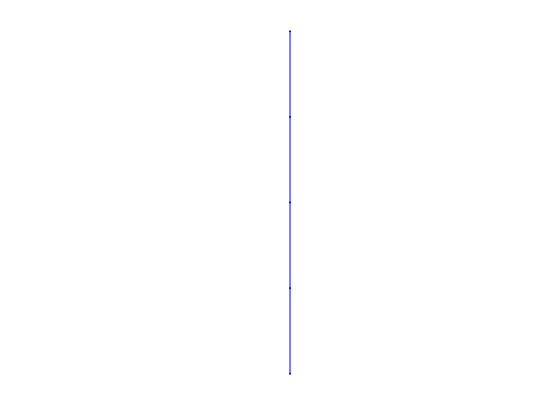
\includegraphics[width=\textwidth]{figures/method/trajectory-sampled}
    \caption{Trajectory sampled \# times (TODO)}
  \end{minipage}
  \hfill
  \begin{minipage}[b]{0.4\textwidth}
    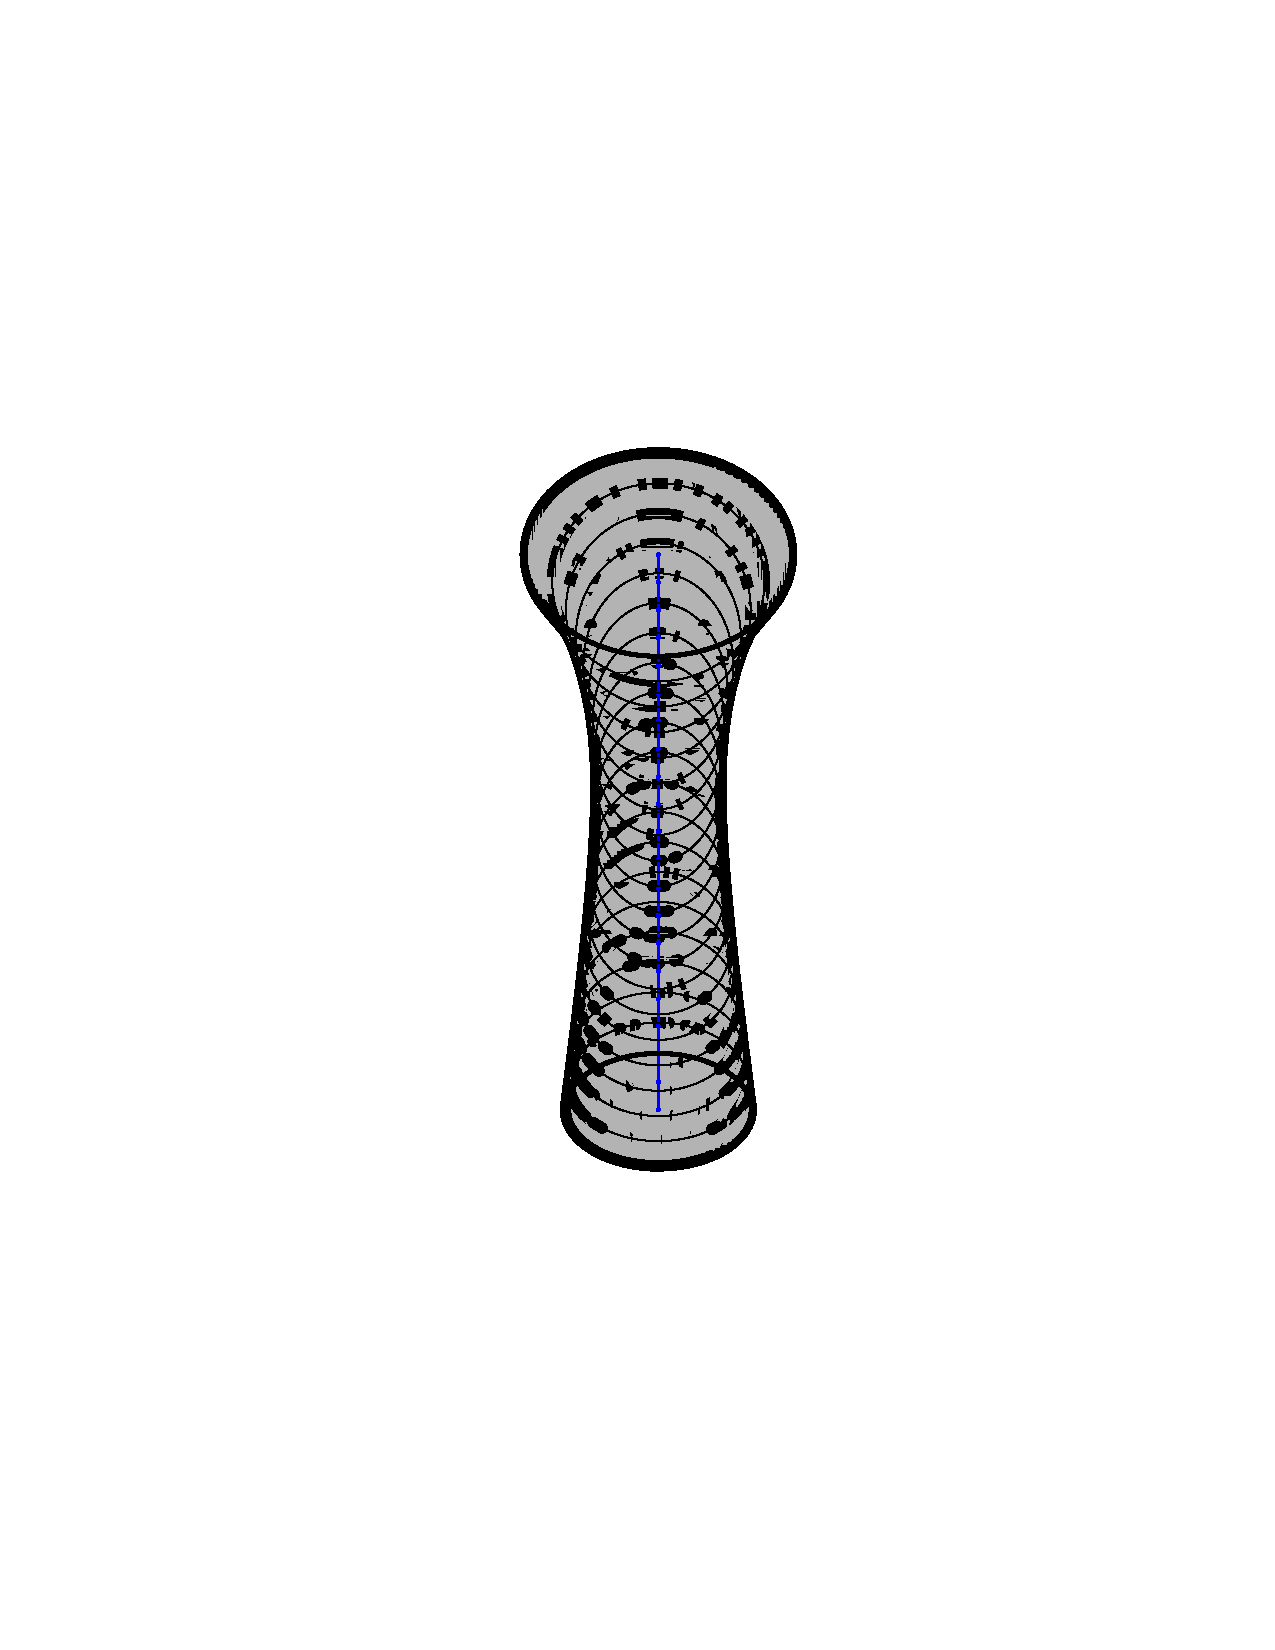
\includegraphics[width=\textwidth]{figures/method/funnel-sampled}
    \caption{The verified trajectory ellipsis overlaid at the sample times.}
  \end{minipage}
\end{figure}

For each funnel, in order to not only be able to compose funnels, but
sub-funnels, which means that at every point of every node in every funnel is
composable with every other sample point in every other funnel has to be
checked. This is summed up more orderly in algorithm
\ref{alg:create-funnel-graph}, where a funnel is a vertice in the graph, and an
ordered pair of funnels \(\left( F_{i}, F_{j} \right)\) is an edge. Composition
of funnels is checked in the same way as in \ref{def:funnel-composition}, and a
\ac{SOS}-program which implements the algorithm can be found
in~(\ref{sec:funnel-composability-program-sos}).

\begin{algorithm}
  \caption{Create Funnel Graph}
  \label{alg:create-funnel-graph}
  \DontPrintSemicolon \SetAlgoNoLine

  \KwIn{\(\mathcal{F}\) -- The basis set of funnels computed around the nominal
    trajectories.} \KwOut{\(\mathcal{G}(\mathcal{F})\) -- Directed graph
    representing the composability of funnels.}

  \ForEach{\(F_{i} \in \mathcal{F}\)} { \ForEach{\(F_{j} \in \mathcal{F}\)} {
      \ForEach{\(t_{k} \in F_{i}\)} { \ForEach{\(t_{l} \in F_{j}\)} {
          \If{\(F_{i}(t_{k}) \subset F_{j}(t_{l})\)} { \(\mathcal{G}
            \leftarrow{} \left( F_{i}(t_{k}), F_{j}(t_{l}) \right)\) } \; } \; }
      \; }\; }\;

\end{algorithm}

Hereafter the primities at each point can be prioritized by some metric, say
distance to the goal or similar.

\subsection{Verify that the vehicle stays within the funnels}

Below is a figure of N simulation runs with the model vehicle in all K of the
funnels from the basis set.

TODO - create figure.


\section{RRT-section}

\subsection{The \rrtfunnel{} algorithm}

The \rrtfunnel{} algorithm is a modified \ac{RRT} graph algorithm which employs
the precomputed funnels as motion primitives for it's expansion operator.

\begin{algorithm}
  \caption{Check funnel composability}
  \label{alg:create-funnel-graph}
  \DontPrintSemicolon \SetAlgoNoLine

  \KwIn{\(\mathcal{F}\) -- The basis set of funnels computed around the nominal
    trajectories.} \KwOut{\(\mathcal{G}(\mathcal{F})\) -- Directed graph
    representing the composability of funnels.}

  \ForEach{\(F_{i} \in \mathcal{F}\)} { \ForEach{\(F_{j} \in \mathcal{F}\)} {
      \If{\(F_{i}(t_{0}) \subset F_{j}(t_{end})\)} { \(\mathcal{G} \leftarrow{}
        \left( F_{i}(t_{0}), F_{j}(t_{end}) \right)\) } \; }\; }\;

\end{algorithm}

\begin{figure}
  \centering 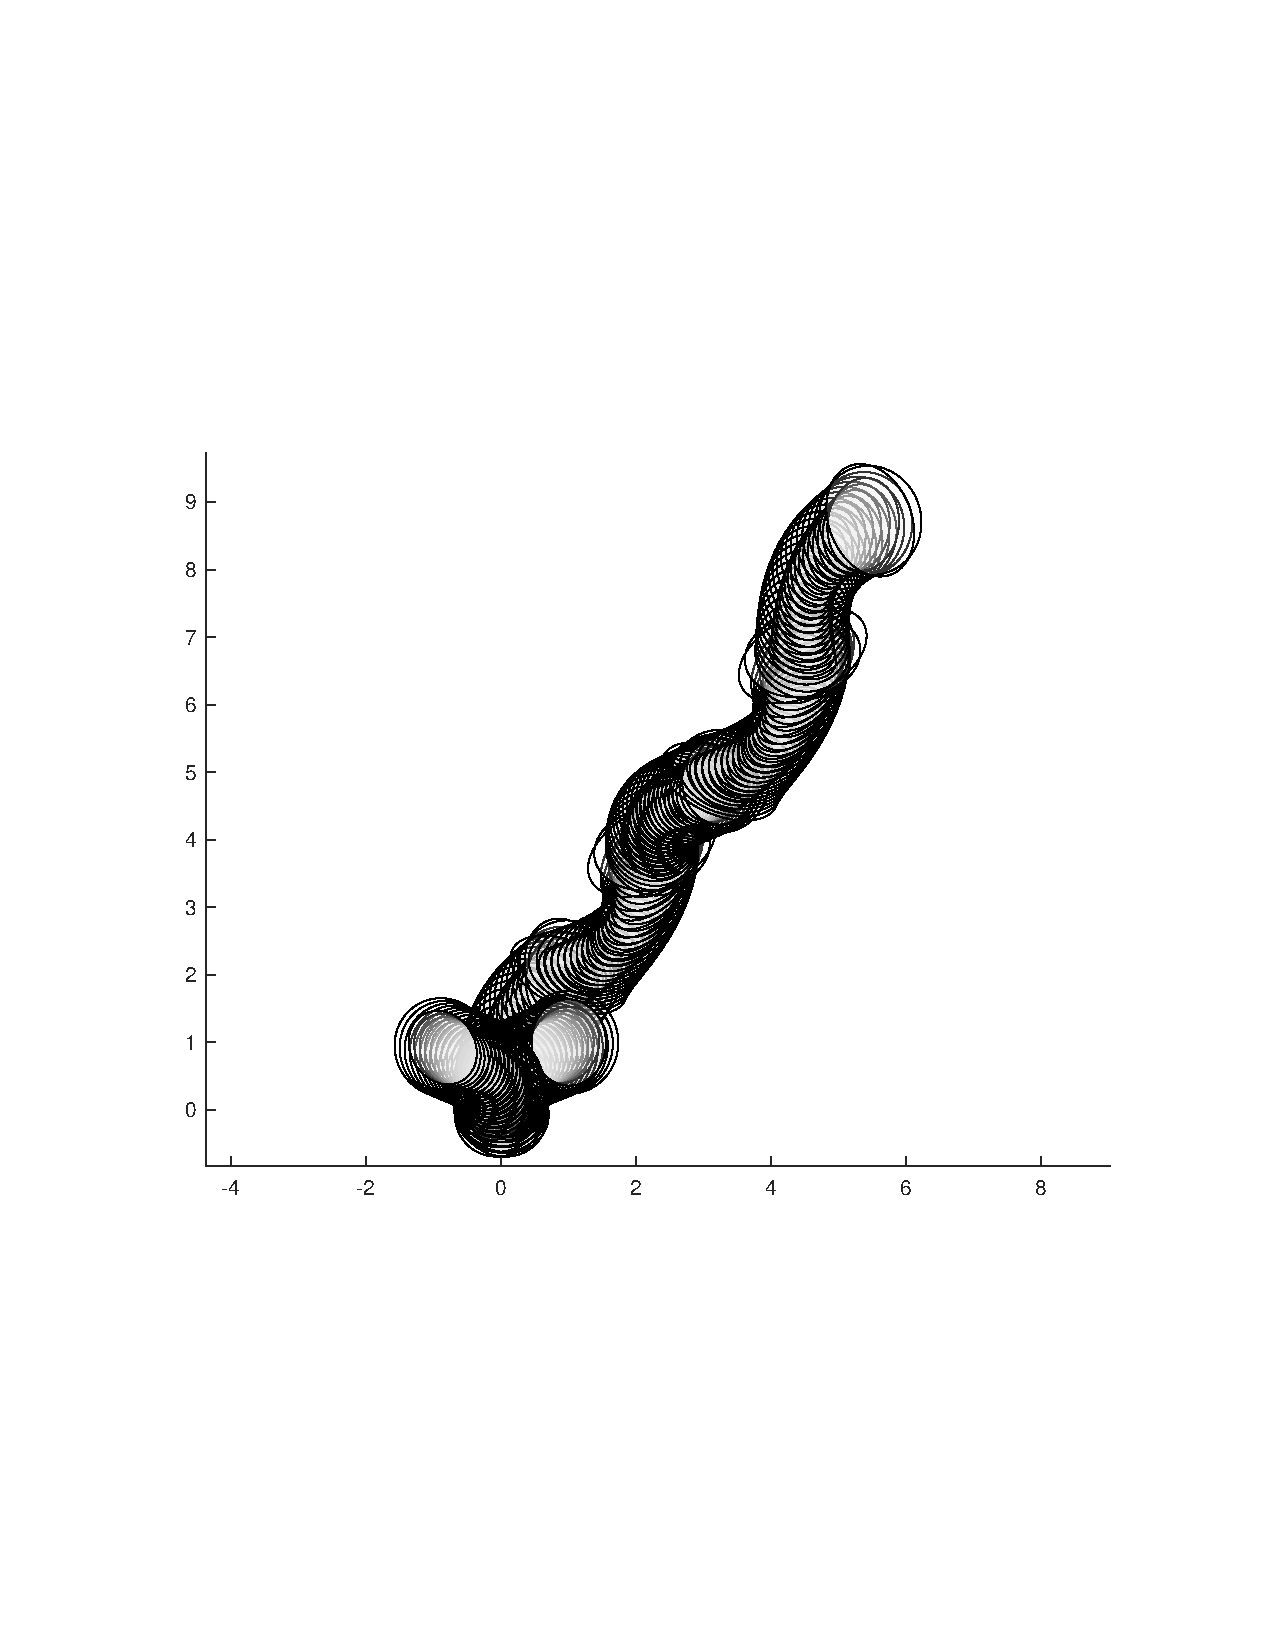
\includegraphics[scale=.5]{figures/method/funnel-tree}
  \caption{Picutred: A tree of funnels built by the \rrtfunnel{} algorithm.}
\end{figure}

The \rrtfunnel{} algorithm is defined as


\begin{algorithm}[H]
  \caption{\rrtfunnel{} algorithm}

  \DontPrintSemicolon

  \KwIn{Initial configuration, \(q_0\)} \KwOut{\textit{RRT}-Funnel-graph
    \(\mathcal{G}\)}

  \SetKwFunction{RandConf}{Sample\_Random\_Configuration}
  \SetKwFunction{NearestVertex}{Find\_Nearest\_Vertex}
  \SetKwFunction{Extend}{Extend} \SetKwFunction{AddVertex}{add\_vertex}
  \SetKwFunction{AddEdge}{add\_edge}
  \SetKwFunction{ExtractBranch}{Extract\_Branch}
  \SetKwFunction{TestUncertainFunnels}{Test\_Uncertain\_Funnels}
  \SetKwFunction{BuildComposabilityMatrix}{Build\_Composability\_Matrix}

  \TestUncertainFunnels{}
  \BuildComposabilityMatrix{}

  \(\mathcal{G}.init(q_0)\) \For{\(i \leftarrow 1\) \KwTo \(k\)}{ \(q_{rand}
    \leftarrow \) \RandConf{} \; \(q_{near} \leftarrow \)
    \NearestVertex{\(q_{rand}, \mathcal{G}\)}\; \(q_{new} \leftarrow \)
    \Extend{\(q_{near}, q_{rand} \)}\; \If{\(q_{new} \in
      \modelconfigurationspacefree{} \) } {
      \(\mathcal{G}\).\AddVertex{\(q_{new}\)}\;
      \(\mathcal{G}\).\AddEdge{\(q_{near}, q_{new}\)} \; \If{\(q_{new} \in
        \mathcal{X}_{goal}\)}{ return \ExtractBranch{\(\mathcal{G}\)} \; }\; } }

  \SetKwProg{Def}{def}{:}{end} \Def{\RandConf{}}{ return 0\; }
  \Def{\TestUncertainFunnels{}}{ return 0\; }
  \Def{\BuildComposabilityMatrix{}}{ return 0\; }
  \Def{\NearestVertex{\(q_{rand}, \mathcal{G}\)}}{ return 0\; }
  \Def{\Extend{\(q_{near}, q_{rand} \)}}{ return 0\; }

  \Def{\ExtractBranch{}}{ return 0\; }

\end{algorithm}

\subsection{The convergence of the algorithm}

The convergence rate \(\epsilon\) is set to 1 percent.

No input saturations modelled.

\subsection{Special maneuvers}
(Maybe have this along with the identity funnel)

\subsubsection{The identity funnel for starting the simulation fresh}

The identity funnel is an empty placeholder for the start node of the graph,
that does no transformations on the model at all, and thus can be seen as the
identity element in the funnel space, or rather, the identity funnel.

\subsubsection{Emergency maneuver}

If the vehicle is to leave the verified funnel at execution time -- this could
happen for any number of reasons, such as unmodelled uncertainties -- the
vehicle should execute the emergency maneuver, which in this case is a simple
stop maneuver. Since the model employed is a simple first order model, a halt
will happen momentarirly. Still, an emergency maneuver can be any sort of 'safe'
maneuver for the model at hand -- such as a loiter circle for an airplane, or
idling at one place for a quadcopter.


\subsection{Alternative to the emergency maneuver}

If the vehicle leaves the current funnel, maybe an idea would be to replan, ie
translate the funnel so that the current state is once again contained within
the funnel, and restart the driving?


\subsubsection{How to obtain uniform sampling}
\subsubsection{How to define a good distance metric}
In general, it is not possible to get a perfect distance metric for our planning
problem, as this involves solving another optimal planning problem, and will
therefore be as, or more complex than the motion planning problem which is
already being solved. Therefore in general we will have to limit ourselves to
approximate distance metrics. The idea is to get as close to the optimal
cost-to-go function without having to compute expensive
computations~\cite{Lav06}. Distance metrics candidates in the RRT-Funnel
algorithm:
\begin{itemize}
\item Time - Since time can be found by simple summing up the time of all the
  funnels which need be added to get to the certain point in the configuration
  space.
\item Lyapunov function - As the Lyapunov function can be seen as an energy
  function, the cost to go to a point can (probably) be used as a metric in the
  planning.
\item Length of the shortest path between two configurations - ignoring
  collisions.
\item A* search heuristics.
\item Geometric - Stacking Funnels, where the shortest funnel of funnels wins.
  e.g. if the point is not in the cone projected out from the current state by
  the current motion primitives, pick the most extreme turn, and start over once
  again. If it can be reached by a turn, turn, then go straight for N-Funnels.
\end{itemize}

Note that most of these metrics are not metrics in the full sense, as they do
not fulfill the symmetric property, as under dynamic constraints going from a to
b, may not be the same as going from b to a. In most cases it is not true for a
nonholonomic vehicle.

\subsubsection{How to extend the tree?}

Should it be expanded into the dynamic Voronoi regions? If so, what are these
regions?

The extend operation can take a different extension or distance metric than the
closest node operation. Maybe this should be used for the benchmark planner. An
extension heuristic which maximizes the distance to the closest trees.

\subsubsection{Sampling with a bias}

Extending with a goal bias of 5 percent is currently used in the \rrtfunnel{}
algorithm. 